\chapter{Analyse}\label{sec:analyse}

\section{Systemsekvensdiagram}
\todo{write stuff about SSD}
\begin{figure}
    \centering
    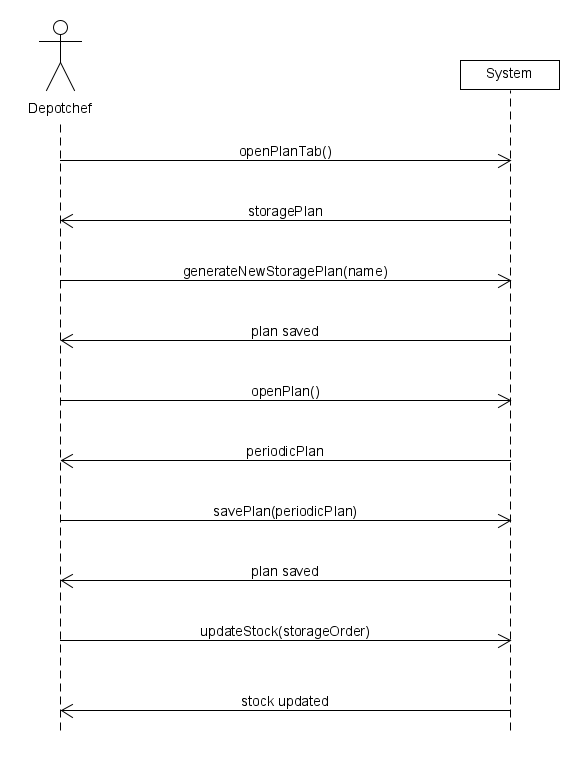
\includegraphics[width=\textwidth]{figures/analyse/SSD.png}
    \caption{Systemsekvensdiagram}
    \label{fig:ssd}
\end{figure}


\section{Operationskontrakt}
\todo{write stuff about operationskontrakt}
%remember to talk about the autogeneration continuation process thing algorithm stuff :) 

\begin{center}
    \begin{longtable}{ |p{360pt}| }
        \hline
        \textbf{Operationskontrakt}
        \\
        \noindent\fbox{%
            \parbox{4.88in}{%
                \textbf{Operation:} openPlanTab() Åbner planfanen i programmet
                
            }%
        }

        \noindent\fbox{%
            \parbox{4.88in}{%
                \textbf{Operation:} generateNewStoragePlan(name) 
                
            }%
        }

        \noindent\fbox{%
            \parbox{4.88in}{%
                \textbf{Operation:} openPlan()
                
            }%
        }
        
        \noindent\fbox{%
            \parbox{4.88in}{%
                \textbf{Operation:} savePlan(periodicPlan)
                
            }%
        }

        \noindent\fbox{%
            \parbox{4.88in}{%
                \textbf{Operation:} updateStock(storageOrder)
                
            }%
        }
        
    \end{longtable}
\end{center}